% A simple linear model
% Ordinary Least Squares (OLS)
% Regression output
% Practice
  % Example: QOG dataset
  % Practice session
  % Exercise

\documentclass[t]{beamer}
\usetheme{\usetheme{hkllite}}

\title{regression}
	\author{François Briatte \& Ivaylo Petev}
	\date{Week~\#8}

\begin{document}
	
    \frame[plain]{
		\titlepage\\[7em]
		\tableofcontents[hideallsubsections]
		}

	%
	%

	% --- prologue: electoral forecasts with data (Silver) or a model (Hibbs)

	\begin{frame}[c]%{``538'' forecast}
				 
		\begin{columns}[T]
		\column{.45\textwidth}

			\href{http://fivethirtyeight.blogs.nytimes.com/}{%
				%
				
\includegraphics[width=\textwidth]{538-logo}\\%
				%
				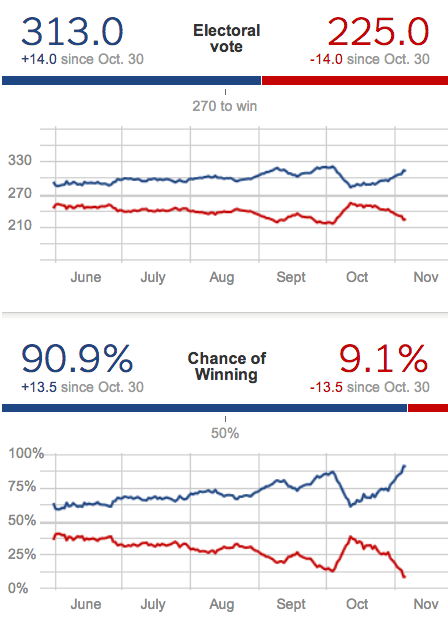
\includegraphics[width=\textwidth]{538-nov6-prediction}%
			}
		
		\column{.4\textwidth}

			\href{http://simplystatistics.org/post/35187901781/nate-silver-does-it-again-will-pundits-finally-accept}{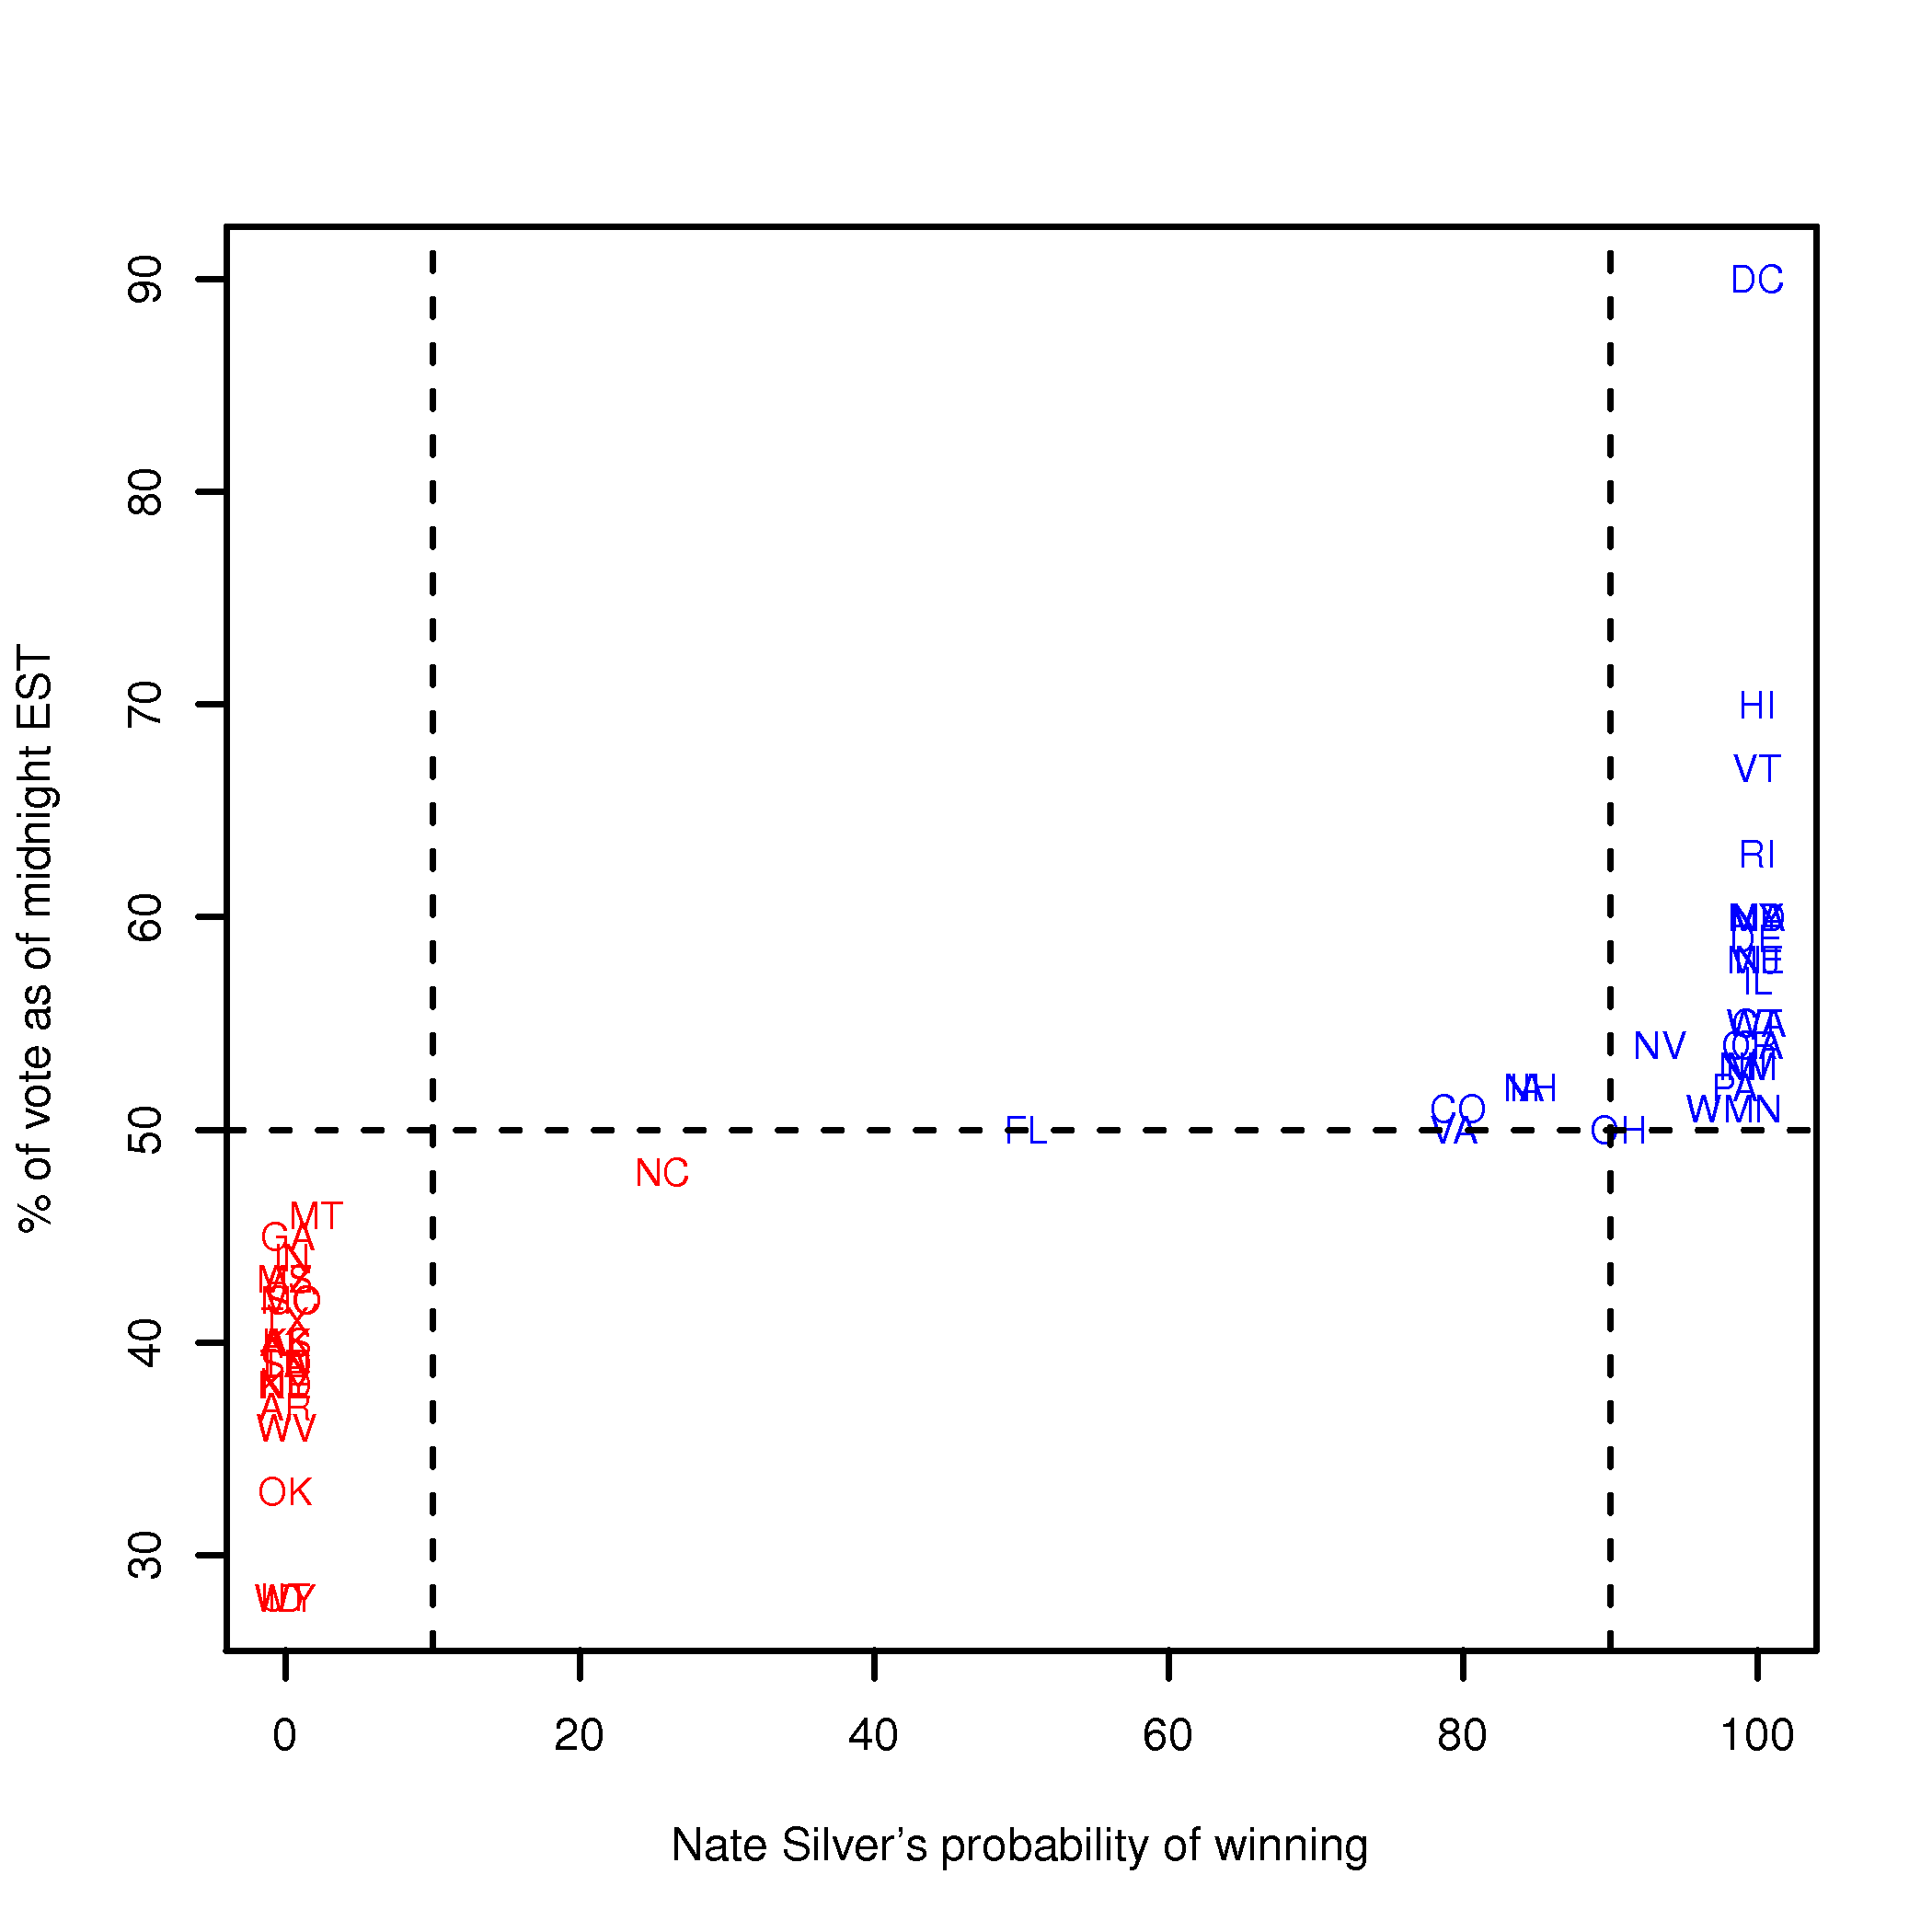
\includegraphics[width=\textwidth]{538-simply-statistics}}
			
			\href{http://www.acthomas.ca/comment/2012/11/538s-uncertainty-estimates-are-as-good-as-they-get.html}{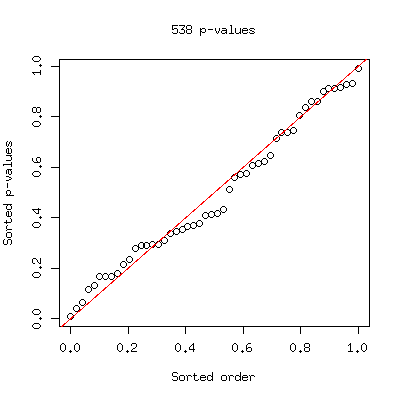
\includegraphics[width=\textwidth]{538-uniform-plots}}
		
		\end{columns}
		
	\end{frame}
	
	\begin{frame}[c]%{``Bread and Peace'' model}
			
		\begin{center}
			\href{http://www.douglas-hibbs.com/HibbsArticles/Web-2012-Post-mortem.htm}{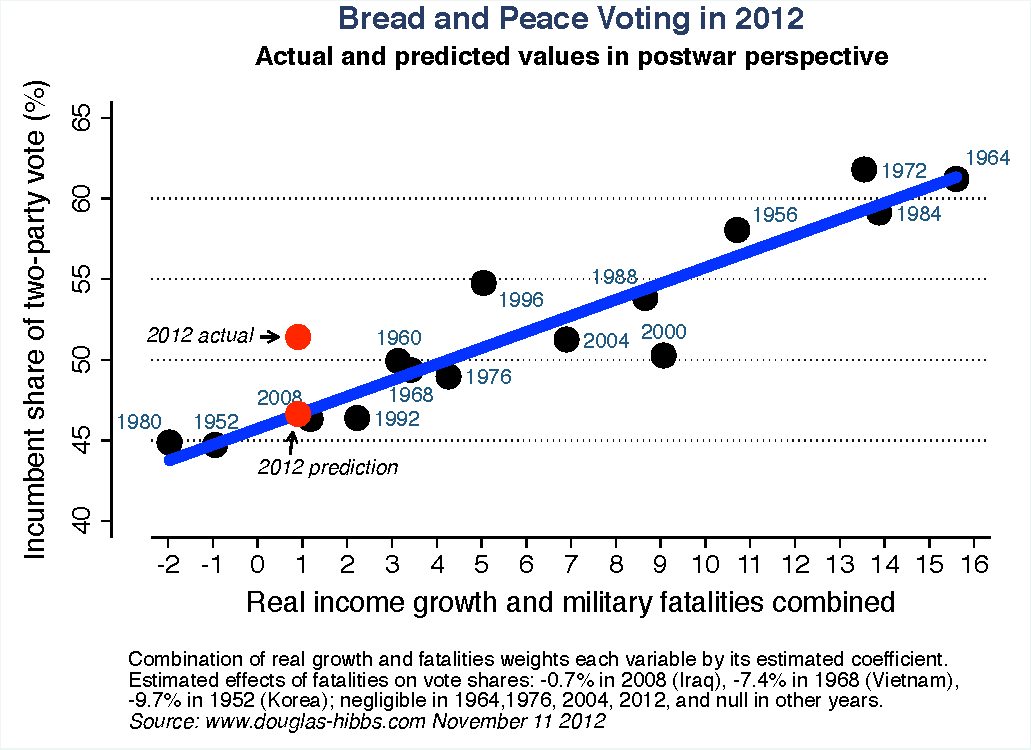
\includegraphics[height=6.5cm]{Hibbs-Post-mortem}}
		\end{center}
				
	\end{frame}

	%
	%
	
	\section{A simple linear model} % A serious man
	
	
	\begin{frame}[c]{}
		
		\vfill

		To what extent can trust in government be predicted from variations in economic growth?
		
		\vfill
		 
		\begin{columns}[T]
		\column{.6\textwidth}

		\begin{block}{DV: Trust in government}

			``Just about always/Most of the time'' (\href{http://www.electionstudies.org/}{American National Election Studies})

		\end{block}

		\begin{block}{IV: Economic performance}

			Change in per capita disposable income (\href{http://www.bea.gov/}{Bureau of Economic Analysis})

		\end{block}

		\vspace{1em}
		\footnotesize{%
			\textit{\href{http://www.themonkeycage.org/2010/02/what_will_make_people_love_gov.html}{Example and data provided by John Sides.}}%
		}

		\column{.35\textwidth}

		
\includegraphics[scale=.4]{obama}
		\end{columns}
		
	\end{frame}
	
	%
	%
	
	% -- correlations

	\begin{frame}[c] % dots
			
		\begin{center}
			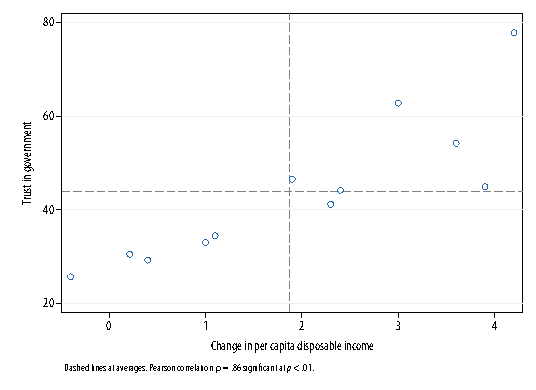
\includegraphics[width=\textwidth]{trust-correlation-0}
		\end{center}
				
	\end{frame}

	\begin{frame}[c] % years
			
		\begin{center}
			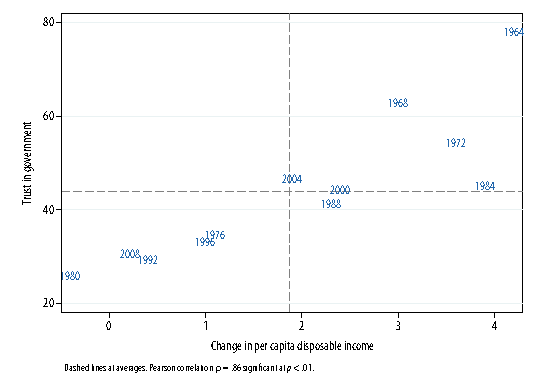
\includegraphics[width=\textwidth]{trust-correlation-1}
		\end{center}
				
	\end{frame}

	\begin{frame}[c] % president/party
			
		\begin{center}
			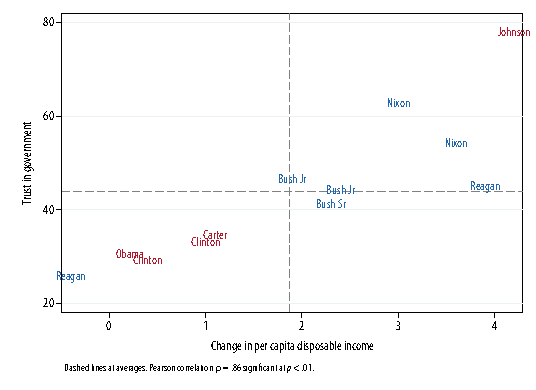
\includegraphics[width=\textwidth]{trust-correlation-2}
		\end{center}
				
	\end{frame}
		
	%
	%
	
	\begin{frame}{Simple linear regression}
		 
		\begin{block}{Equations}
			$Y = \alpha + \beta X + \epsilon \quad \hat{Y} = \hat{\alpha} + \hat{\beta} X + \hat{\epsilon} \quad \epsilon = Y - \hat{Y}$
		\end{block}
		
		\begin{block}{Parameters}
			\begin{itemize}
			 	\item $Y$ is the dependent variable and $\hat{Y}$ its predicted value
			 	\item $X$ is the independent variable used as a predictor of $Y$
			 	\item $\alpha$ is the \red{constant} (intercept)
			 	\item $\beta$ is the \red{regression coefficient} (slope)
			 	\item $\epsilon$ is the \red{error term} (residuals)
			\end{itemize}
		\end{block}

		\begin{alertblock}{Warning}
		 	The model assumes a \emph{linear}, \emph{additive} relationship.
		\end{alertblock}
		
	\end{frame}

	%
	%

	% -- linear fits

	\begin{frame}[c] % dots
			
		\begin{center}
			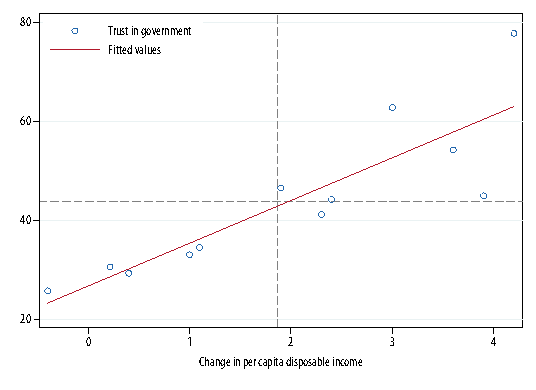
\includegraphics[width=\textwidth]{trust-linear-fit-1}
		\end{center}
				
	\end{frame}

	\begin{frame}[c] % years
			
		\begin{center}
			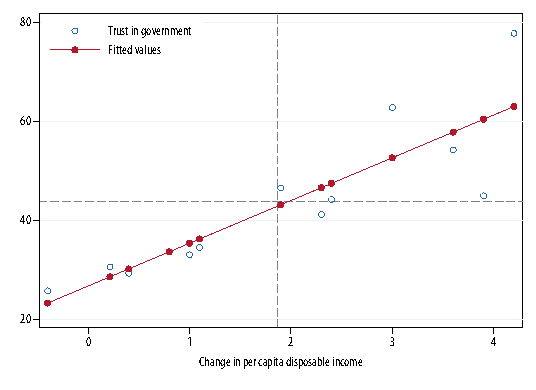
\includegraphics[width=\textwidth]{trust-linear-fit-2}
		\end{center}
				
	\end{frame}

	\begin{frame}[c] % president/party
			
		\begin{center}
			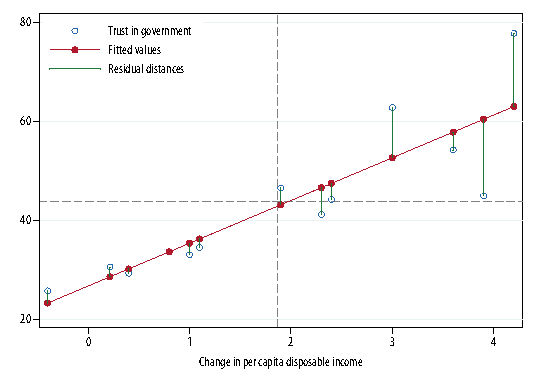
\includegraphics[width=\textwidth]{trust-linear-fit-3}
		\end{center}
				
	\end{frame}
	
	%
	%
	
	\section{Ordinary Least Squares (OLS)}

	\begin{frame}[c]{Ordinary Least Squares (OLS)}
		
		\begin{block}{Error term}

		In a simple linear model $Y = \alpha + \beta X + \epsilon$, the regression coefficient $\beta$ is calculated as to minimize the \red{residual sum of squares}

		$$RSS = \sum _{i=1} ^n (Y_i - \hat{Y_i})^2 = \sum _{i=1} ^n \epsilon^2$$

		where $Y_i - \hat{Y_i}$ is the residual (or error term) of each observation.
		\end{block}
		
		\begin{block}{Parameter estimation}
			$$\beta = \frac{\text{Cov}(X,Y)}{\text{Var}_X} = \frac{\sum ^n _{i=1}(X_i - \bar{X}) (Y_i - \bar{Y})}{\sum ^n _{i=1}(X_i - \bar{X})^2} \quad \alpha = \bar{Y} - \beta\bar{X}$$
		\end{block}
				
	\end{frame}

	% -- residuals

	% \begin{frame}[c] % dots
	% 		
	% 	\begin{center}
	% 		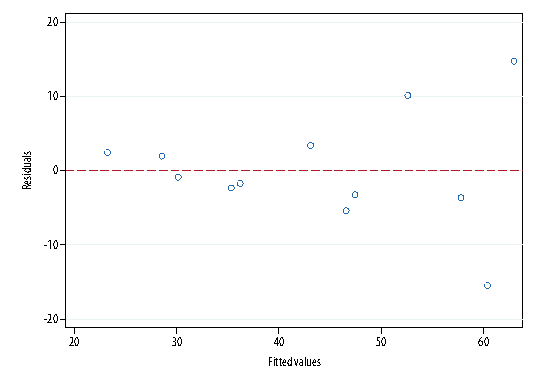
\includegraphics[width=\textwidth]{trust-residuals-0}
	% 	\end{center}
	% 			
	% \end{frame}
	% 
	% \begin{frame}[c] % years
	% 		
	% 	\begin{center}
	% 		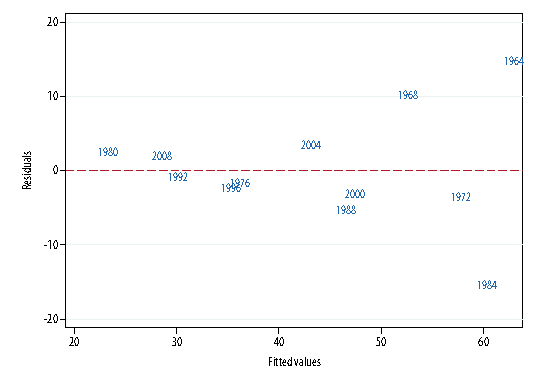
\includegraphics[width=\textwidth]{trust-residuals-1}
	% 	\end{center}
	% 			
	% \end{frame}
	% 
	% \begin{frame}[c] % president/party
	% 		
	% 	\begin{center}
	% 		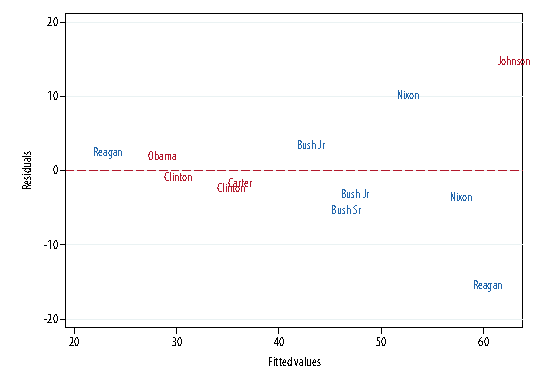
\includegraphics[width=\textwidth]{trust-residuals-2}
	% 	\end{center}
	% 			
	% \end{frame}

	%
	%

	\section{Regression output}
				
	\begin{frame}[t]{\texttt{reg y x}}

	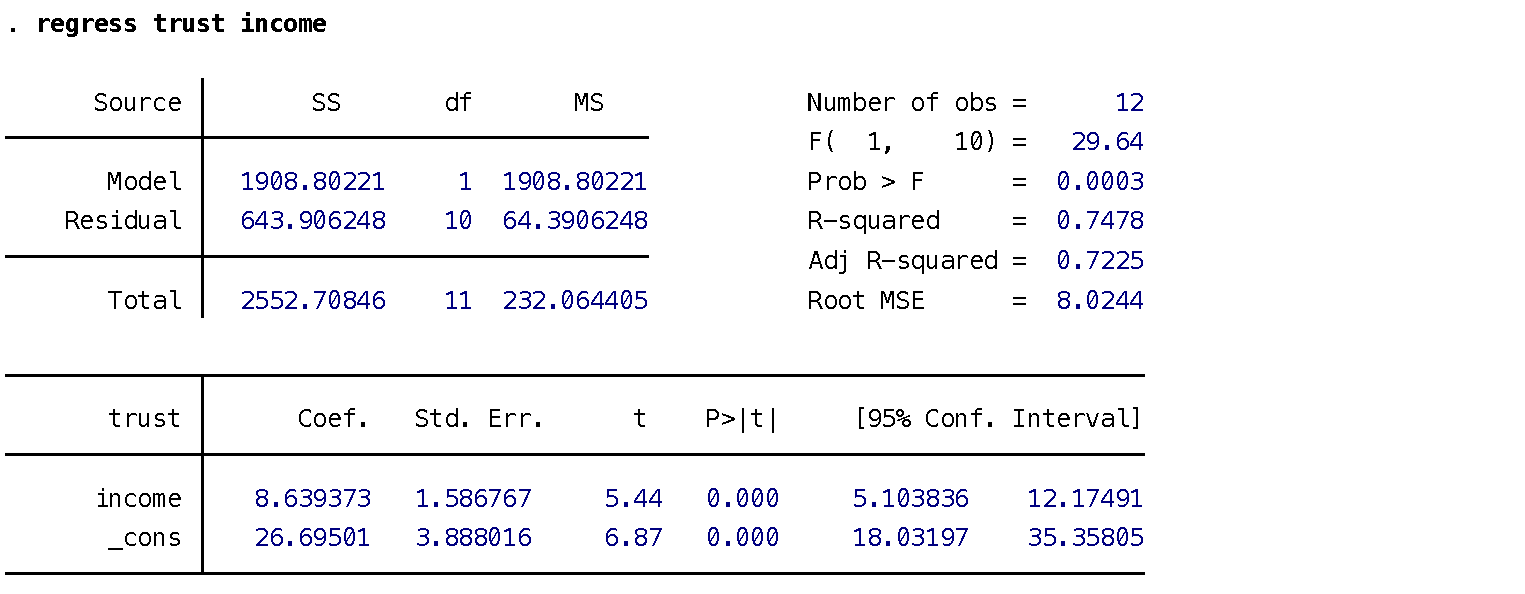
\includegraphics[width=\textwidth]{reg-out-0.pdf}
	
	Top left: ANOVA table. Top right: model fit.
	
	Bottom: regression coefficients.
	
	\end{frame}

	%
	%

	\begin{frame}[t]{Interpretation of fit}

	\begin{columns}[T]

	\column{.65\textwidth}

	Number of observations $N$, significance test $H_0: \beta = 0$, coefficient of determination $R^2$, \red{root mean square error} (RMSE).\\[1em]

	\begin{block}{Goodness of fit}\vspace{.5em}
		$R^2 = 1 - \frac{\sum ^n _{i=1}(\red{Y_i} - \hat{Y_i})^2}{\sum ^n _{i=1}(\red{Y_i} - \bar{Y_i})^2} \color{gray}{ = \frac{\text{residual sum of squares}}{\text{total sum of squares}}}$\\[1em]

		As the fit improves, $RSS \to 0$ and $R^2 \to 1$.
	\end{block}

	\begin{alertblock}{Sanity check}
		Focus on getting $N$ and the RMSE right.
	\end{alertblock}

	\column{.3\textwidth}
		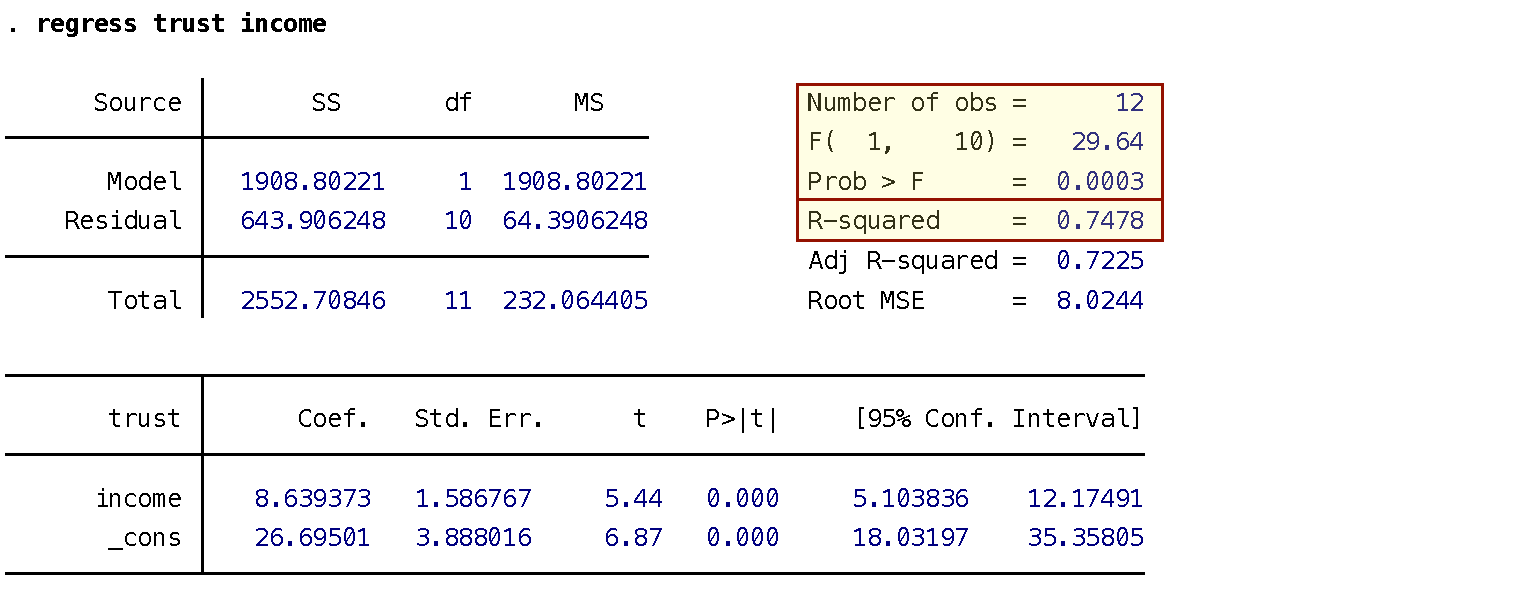
\includegraphics[width=\textwidth]{reg-out-1.pdf}\vspace{1cm}
		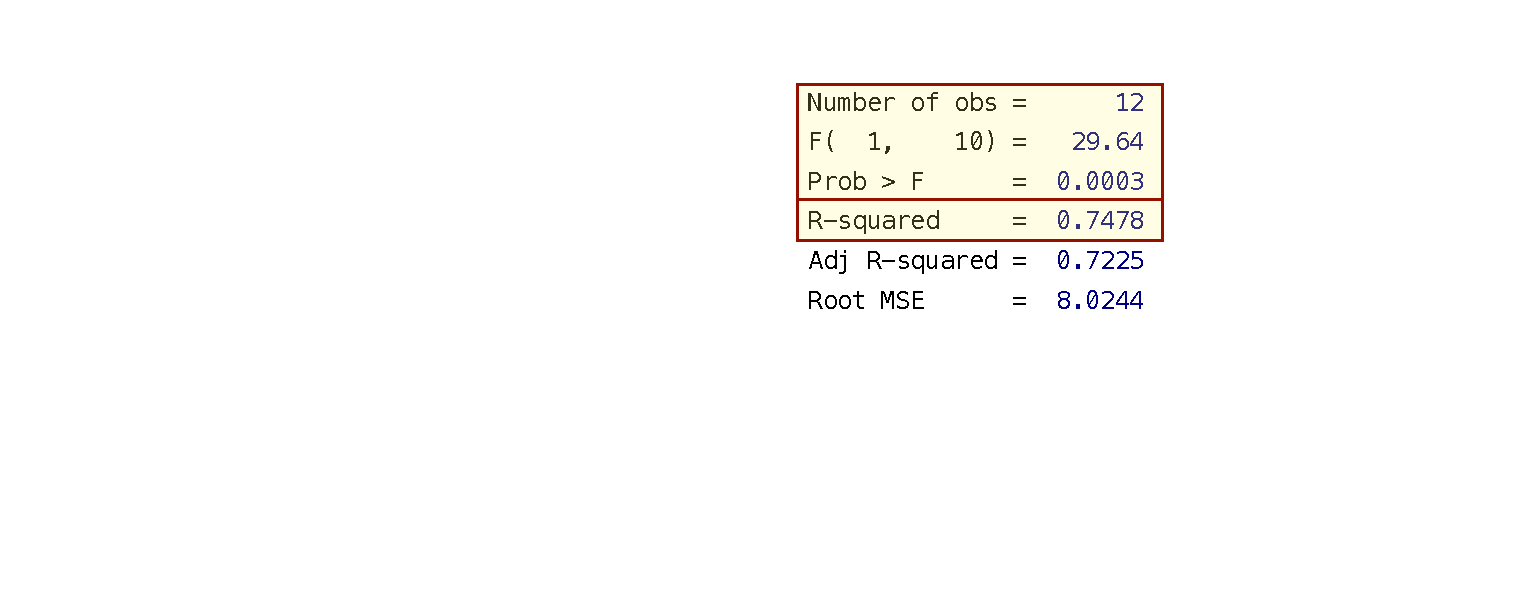
\includegraphics[width=\textwidth]{reg-out-1b.pdf}\vspace{1cm}
	\end{columns}

	\end{frame}

	\begin{frame}[t]{Interpretation of regression coefficients}

	\begin{columns}[T]

	\column{.65\textwidth}	

	A regression coefficient estimates the variation in $Y$ predicted by a change in one unit of $X$ \color{gray}{(recall that $Y = \alpha + \beta X + \epsilon$)}

	\column{.3\textwidth}
		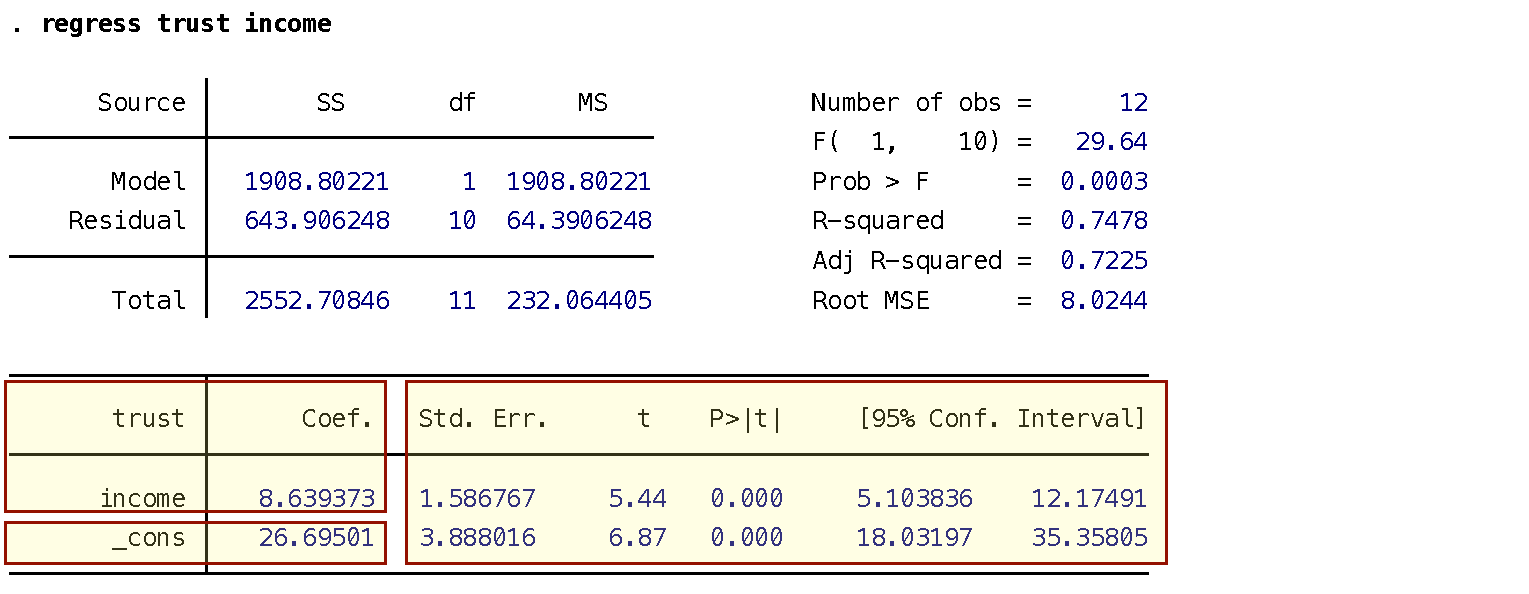
\includegraphics[width=\textwidth]{reg-out-2.pdf}\vspace{1cm}
	\end{columns}

	\vspace{-1em}
	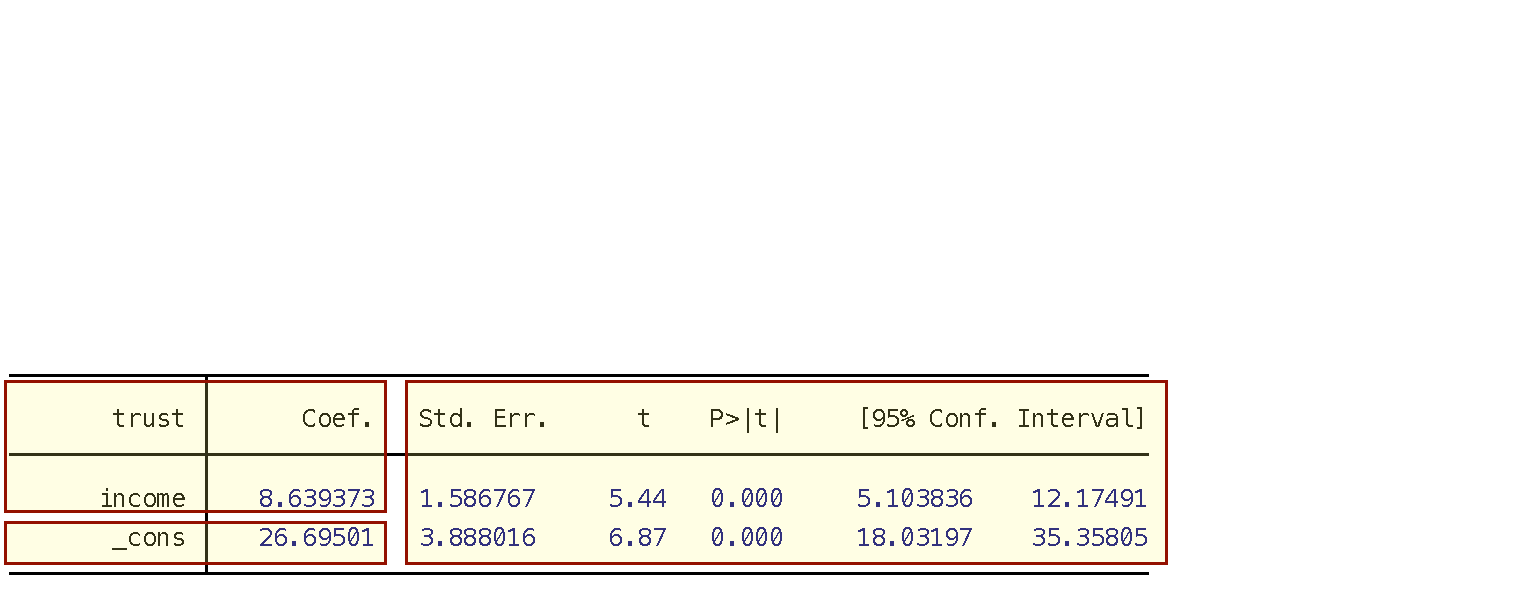
\includegraphics[width=\textwidth]{reg-out-2b.pdf}%\vspace{.5em}

	\begin{itemize}
		\item The \red{coefficient} is the slope $\beta$ of the regression line and the \red{constant} is its intercept, the coordinate of origin $\alpha = \hat{Y}_{X=0}$.

		\item The \red{standard error}, $t$-value and $p$-value test whether the coefficient is significantly different from $0$.
	\end{itemize}

	\end{frame}

	\begin{frame}[c]{Logarithmic coefficients: see \href{http://www.ats.ucla.edu/stat/mult_pkg/faq/general/log_transformed_regression.htm}{UCLA mini-guide}}
	
		\begin{block}{Linear-linear relationships: $Y = \alpha + \beta X$}
			An increase of one unit of $X$ is associated with an increase of $\beta_1$ units of $Y$.
		\end{block}
	
		\begin{block}{Log-linear relationships: $\red{\ln Y} = \alpha + \beta X$}
			An increase of one unit of $X$ is associated with a $100 \times \beta_1$\% increase in $Y$ (true effect: $Y \times$ \texttt{exp($\beta_1$)}).
		\end{block}

		\begin{block}{Linear-log relationships: $Y = \alpha + \red{\beta \ln X}$}
			A 1\% increase in $X$ is associated with a $0.01 \times \beta_1$ unit increase in $Y$ (e.g. $\beta_1 \times$ \texttt{log(1.15)} for +15\% in $X$).
		\end{block}
	
		\begin{block}{Log-log relationships: $\red{\ln Y} = \alpha + \red{\beta \ln X}$}
			A 1\% increase in $X$ is associated with a $\beta_1$\% increase in $Y$.
		\end{block}
	
	\end{frame}
	
	%
	%

	\begin{frame}[c]{Factor coefficients}
	
		\begin{block}{\code{reg trust income \red{i.republican}}}
			
			\begin{itemize}
				\item For Democrat presidents, \texttt{republican == 0}
				
				$$Y = \alpha + \beta X_0 = \alpha$$
				
				\item For Republican presidents, \texttt{republican == 1}
				
				$$Y = \alpha + \red{\beta X_1}$$
				
			\end{itemize}
						
		\end{block}
		
		\begin{block}{Dummies in regression equations}
			
			\begin{itemize}
			
				\item The first category (0) is used as the `baseline' and is omitted.
				\item This logic applies to any variable passed to \code{reg} with \code{i.}

			\end{itemize}
			
		\end{block}
	
	\end{frame}
	%
	%
	
	% \section{Draft No.~2}
	% 
	% \begin{frame}[t]{Draft No. 2}
	% 
	% \begin{columns}[T]
	% \column{.3\textwidth}
	% \textbf{Univariate\\statistics}
	% 
	% \vspace{.55em}
	% \begin{itemize}
	% 	\item Introduction
	% 	% (analysis of survey data)
	% 	\item Datasets
	% 	% (observations and variables)
	% 	\item Distributions
	% 	% (central tendency, variability, normality)
	% 	\item Estimation
	% 	% (PDF, CLT, LLN, CI, MLE)
	% \end{itemize}
	% Assignment No. 1
	% 
	% $$
	% \left.
	%     \begin{array}{rrr}
	%         corrected \\
	%         revised\\
	%         appended
	%     \end{array}
	% \right \} 
	% $$
	% 
	% \column{.3\textwidth}
	% \textbf{Bivariate\\statistics}
	% 
	% \begin{itemize}
	% 	\item Significance
	% 	% (t-test, comparison of means and proportions)
	% 	\item Crosstabs
	% 	% (Chi-squared test)
	% 	\item Correlation
	% 	% (scatterplot and correlation matrixes)
	% 	\item Simple OLS
	% 	% (Simple OLS linear regression)
	% \end{itemize}
	% \red{Assignment No. 2}\\[.5em]
	% 
	% \fbox{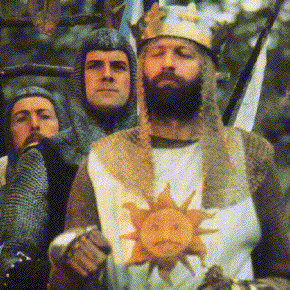
\includegraphics[width=.75\textwidth]{holy-grail2.jpg}}
	% 
	% \column{.3\textwidth}
	% \textbf{Statistical\\modelling}
	% 
	% \begin{itemize}
	% 	\item Regression
	% 	% (residuals)
	% 	\item Extensions
	% 	% (dummies)
	% 	\item Diagnostics
	% 	% (multicollinearity, heteroscedasticity)
	% 	\item Conclusion
	% 	% (GLS, logistic, ANOVA, Bayesian...)
	% \end{itemize}
	% Final paper\\[.5em]
	% \fbox{
\includegraphics[width=.75\textwidth]{holy-grail.jpg}}
	% \end{columns}
	% 
	% \end{frame}
	% 
	% %
	% %
	% 
	% \begin{frame}[t]{First steps}
	% 
	% \begin{block}{Revise Draft No.~1}
	% 	
	% 	\begin{itemize}
	% 		\item go through corrections
	% 		\item remove technical content
	% 		\item \red{rewrite until concision}
	% 	\end{itemize}
	% 
	% \end{block}
	% 
	% \begin{block}{Explore associations}
	% 	
	% 		\begin{itemize}
	% 			\item between DV and IVs
	% 			\item between two IVs
	% 		\end{itemize}
	% 
	% 		Write up \red{substantive results} as sentences; cite significance tests and other statistics in brackets, e.g. ($\rho = .7, p < .05$).
	% \end{block}
	% 
	% \end{frame}
	% 
	% %
	% %
	% 

		% 	    \section{Draft No. 2}
		% 
		% 	    \begin{frame}[t]{Where we are now}
		% 
		% 	    \begin{columns}[T]
		% 	    \column{.3\textwidth}
		% 	    \textbf{Univariate\\statistics}
		% 
		% 	    \vspace{.55em}
		% 	    \begin{itemize}
		% 	        \item Introduction
		% 	        \item Dataset
		% 	        \item Variables
		% 	    \end{itemize}
		% 
		% 	    Assignment No. 1
		% 
		% 	    $$
		% 	    \left.
		% 	        \begin{array}{rrr}
		% 	            corrected \\
		% 	            revised\\
		% 	            appended
		% 	        \end{array}
		% 	    \right \}
		% 	    $$
		% 
		% 	    \column{.3\textwidth}
		% 	    \textbf{Bivariate\\statistics}
		% 
		% 	    \begin{itemize}
		% 	        \item Associations
		% 	        \item Correlations
		% 	        \item Simple OLS
		% 	    \end{itemize}
		% 	    \red{Assignment No. 2}\\[.5em]
		% 
		% 	    \fbox{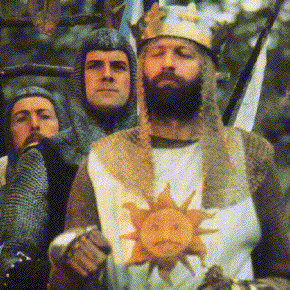
\includegraphics[width=.75\textwidth]{holy-grail2.jpg}}
		% 
		% 	    \column{.3\textwidth}
		% 	    \textbf{Statistical\\modelling}
		% 
		% 	    \begin{itemize}
		% 	        \item Regressions
		% 	        \item Diagnostics
		% 	        \item Conclusion
		% 	    \end{itemize}
		% 	    Final paper\\[.5em]
		% 	    \fbox{
\includegraphics[width=.75\textwidth]{holy-grail.jpg}}
		% 	    \end{columns}
		% 
		% 	    \end{frame}
		% 
		% 	    %
		% 	    %
		% 
		% \subsection{Essential instructions}
		% 
		% 	    \begin{frame}[t]{Essential instructions}
		% 
		% 	    \begin{block}{Revise Draft No.~1}
		% 
		% 	        \begin{itemize}
		% 	            \item go through corrections
		% 	            \item remove technical content
		% 	            \item \red{rewrite until concision}
		% 	        \end{itemize}
		% 
		% 	Pay attention to paragraph limits and scientific style (esp. sources).
		% 
		% 	    \end{block}
		% 
		% 	    \begin{block}{Explore associations}
		% 
		% 	            \begin{itemize}
		% 	                \item between DV and IVs (covariates, controls), or between two IVs
		% 			\item with graphs and then with significance tests
		% 	            \end{itemize}
		% 
		% 	            Write up \red{substantive results} as sentences; cite significance tests and other statistics in brackets, e.g. ($\rho = .7, p < .05$).
		% 	    \end{block}
		% 
		% 	    \end{frame}
		% 
		% 	    %
		% 	    %
		% 
		% \subsection{Structure and style}
		% 
		% \begin{frame}[c]{Structure and style}
		% 
		% 		\begin{columns}[T]
		% 			\column{.4\textwidth}
		% 				\href{http://goo.gl/7u8oa}{Paper template} \\[.5em]
		% 				\fbox{%
		% 					%
		% 					
\includegraphics[width=\textwidth]{paper-template}
		% 				}
		% 			\column{.4\textwidth}
		% 				\href{http://onlinelibrary.wiley.com/doi/10.1111/j.1741-3737.2005.00175.x/abstract}{White (2005)} \\[.5em]
		% 				\fbox{%
		% 					
\includegraphics[width=\textwidth]{white-1page}
		% 				}	
		% 		\end{columns}
		% 		
		% 	% \vfill
		% 
		% 	% Source: Journal of Marriage and Family} 67: 791--8, 2005.
		% 
		% 	    \end{frame}

	    %
		%

	    % \begin{frame}[c]{Scientific style}
	    % 
	    %     \begin{block}{Structure}
	    %         The reader must understand where you are going at all stages. Check by trying to read your paragraphs in isolation.
	    %     \end{block}
	    %     
	    %     \begin{block}{Focus}
	    %         The reader must get only what he needs to understand your analysis: no more, no less. Technical notes show only in your do-file.
	    %     \end{block}
	    %         
	    %     \begin{block}{Evidence}
	    %         Every claim that you make must be grounded in the data, except for the data source and brief literature review in your opening sections.
	    %     \end{block}
	    % 
	    %     \begin{block}{Precision}
	    %         `High income' versus `low income' is a simplification. `Blacks have many babies due to cultural standards' is a stereotype.
	    %     \end{block}
	    % 
	    % \end{frame}

	    %
	    %

	% 	\subsection{Help with Stata}
	% 
	% 	\begin{frame}[t,fragile]{The \texttt{stab} command}
	% 
	% 		\begin{block}{Syntax: \texttt{stab using Briatte\_Petev\_1, replace...}}
	% 
	% 	        \begin{itemize}
	% 	            \item \texttt{sum()} summarizes continuous variables
	% 	            \item \texttt{fre()} summarizes categorical variables
	% 	            \item \texttt{by()} creates multiple tables for comparison
	% 	        \end{itemize}
	% 
	% 			Add the \texttt{corr} option to also export a correlation matrix.
	% 
	% 	    \end{block}
	% 
	% 		\begin{exampleblock}{\texttt{use datasets/nhis2009, clear}}%
	% 			\vspace{-1em}
	% 
	% 	        \begin{verbatim}
	% stab using Briatte_Petev_1, replace ///
	%     sum(age weight height) corr ///
	%     fre(sex uninsured health) ///
	%     by(regionbr)\end{verbatim}
	% 
	% 	    \end{exampleblock}
	% 
	% 	\end{frame}

		% \begin{frame}[c]{Stata video tutorials}
		% 
		% 	        \href{https://www.youtube.com/watch?v=AlEmUqMBx4A&feature=plcp}{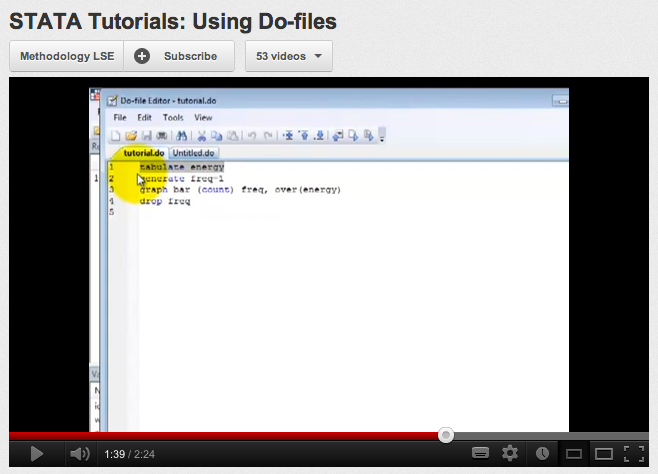
\includegraphics[width=.475\textwidth]{lse-tutorials-1}}%
		% 	\hfill%
		% 	\href{https://www.youtube.com/watch?v=0C_Hlh_jNq8&feature=plcp}{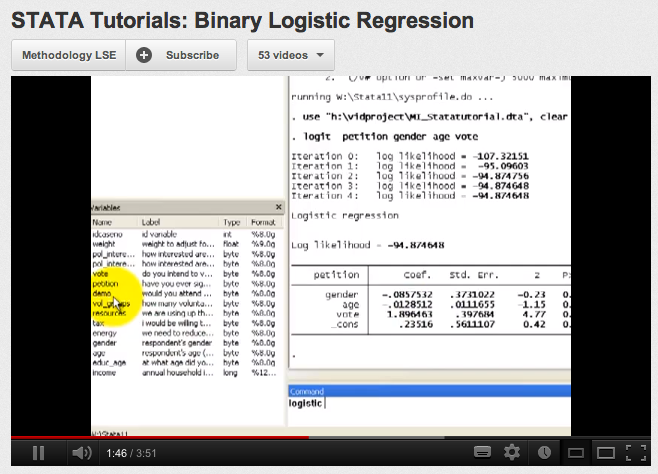
\includegraphics[width=.475\textwidth]{lse-tutorials-2}}%
		% 	%
		% 	\vfill%
		% 	%
		% 	Source: \href{https://www.youtube.com/user/MethodologyLSE/videos?query=stata}{LSE Methodology Institute}, 2012.
		% 
		% 	    \end{frame}

	% \subsection{Coursework}
	% 
	% \begin{frame}[c]{Coursework}
	% 
	% 	\begin{alertblock}{Project \hfill \emph{Stata Guide}, Sec.~13--15}
	% 		\begin{itemize}
	% 			\item Correct and improve Draft No.~1
	% 			\item Finalize association tests and interpretations
	% 			\item Name your paper (\red{PDF}) and do-file like \red{Briatte\_Petev\_2}
	% 		\end{itemize}
	% 	\end{alertblock}
	% 	
	% 	\begin{block}{Readings}
	% 		\begin{itemize}
	% 			\item \emph{Making History Count}, ch.~4 (simple regression)
	% 			\item \emph{Stata Guide}, Sec.~10 (association)
	% 			\item \emph{Stata Guide}, Sec.~11 (correlation and simple regression)
	% 		\end{itemize}
	% 	\end{block}
	% 	
	% 	\vfill Enjoy your day and see you soon!
	% 					
	% \end{frame}

	%
	%
	\section{Practice}
	%	
	%

	%
	%
	\subsection{Example: QOG dataset}
	%
	%
	
	\begin{frame}[t]{Practice: \red{QOG dataset}}

		\begin{columns}[c]
			\column{.55\textwidth}

	    Data:\\[.5em]

			\begin{itemize}
				\item Quality of Government (QOG)
				\item Sample: countries, c.~2002
			\end{itemize}
		
			\vspace{.75em}
		
	    Variables:\\[.5em]
		
			\begin{itemize}
				\item Fertility rate
				\item Education years
				\item Corruption Perceptions Index
				\item Human Development Index
				\item Female ministers
			\end{itemize}
	
			\column{.35\textwidth}

			
\includegraphics[width=\textwidth]{logo-qog}

		\end{columns}
	
	\end{frame}
	%
	%
	
	%
	%
	\subsection{Practice session}
  %
  %
  
	\begin{frame}[t]{Practice session}

    \begin{block}{Class}
      \comm{Get the do-file for this week.}\\
      \code{srqm\_get week8.do}\\
      
			\comm{Open to read and replicate.}\\
			\code{doedit code/week8}\\    
    \end{block}

    \begin{alertblock}{Coursework}
      \begin{itemize}
	      \item Finish the do-file and read all comments at home.
	      \item Correct your do-file and add significance tests.
	      \item Correct your paper and substantiate its hypotheses.
      \end{itemize}
    \end{alertblock}
    		
	\end{frame}
  %
  %
	
  %
  %
  \subsection{Exercise}
  %
  %
  
  \begin{frame}{Exercise}

		\begin{exampleblock}{Ex~8.1. Quality of Government 2011}

			\begin{itemize}
				\item Variables: \texttt{d wdi\_gdpc wdi\_mege wdi\_pb2 wdi\_the}
				\item Plot correlations and estimate simple linear regressions.
			\end{itemize}

		\end{exampleblock}


    \begin{exampleblock}{Ex~8.2. Quality of Government 2011}
			
			\begin{itemize}
				\item Variables: \texttt{d wdi\_pb2 gol\_polreg }
				\item Plot correlations and estimate simple linear regressions, using \texttt{wdi\_pb2}
			\end{itemize}
			
    \end{exampleblock}


  \end{frame}
  %
  %  
	
\end{document}
